% Customizable fields and text areas start with % >> below.
% Lines starting with the comment character (%) are normally removed before release outside the collaboration, but not those comments ending lines

%%%%%%%%%%%%% local definitions %%%%%%%%%%%%%%%%%%%%%


%%%%%%%%%%%%%%%  Title page %%%%%%%%%%%%%%%%%%%%%%%%
%\cmsNoteHeader{XXX-08-000}
%%%%%%%%%%%%%%%%%%%%%%%%%%%%%
% This is over-written in the CMS environment: useful as preprint no. for export versions
% >> Title: please make sure that the non-TeX equivalent is in PDFTitle below for papers. For PASs, PDFTitle can be used with plain TeX.
\title{The Phase-2 Upgrade of the CMS Beam Radiation, Instrumentation, and Luminosity Detectors: Technical Design Report}

% >> Authors
%Author is always "The CMS Collaboration" for PAS and papers, so author, etc, below will be ignored in those cases
%For multiple affiliations, create an address entry for the combination
%To mark authors as primary, use the \author* form
%%%%%%%%%%%%%%%%%%%%%%%%%%%%%%%%%%%

%\address[cern]{CERN}
%\author*[cern]{A. Cern Person}
%%%%%%%%%%%%%%%%%%%%%%%%%%%%%%%%%%
% >> Date
% The date is in yyyy/mm/dd format. Today has been
% redefined to match, but if the date needs to be fixed, please write it in this fashion.
\date{\today}

% >> Abstract
% Abstract processing:
% 1. **DO NOT use \include or \input** to include the abstract: our abstract extractor will not search through other files than this one.
% 2. **DO NOT use %**                  to comment out sections of the abstract: the extractor will still grab those lines (and they won't be comments any longer!).
% 3. For PASs: **DO NOT use CMS tex macros.**...in the abstract: CDS MathJax processor used on the abstract doesn't understand them _and_ will only look within $$. The abstracts for papers are hand formatted so macros are okay.
\abstract{
   Your abstract here.
}

% >> PDF Metadata
% Do not comment out the following hypersetup lines (metadata). They will disappear in NODRAFT mode and are needed by CDS.
% Also: make sure that the values of the metadata items are sensible and are in plain text with the possible exception of the PDFtitle for a PAS. Then you can use pure TeX symbols as if on a typewriter. Examples: $\sqrt{s}=13\TeV$ => $sqrt{s}=$ 13 TeV; 32\fbinv => 32 fb$^{-1}$
% No unescaped comment % characters.
% No curly braces {} except for TeX in the PDFtitle.
\hypersetup{%
pdfauthor={G. Auzinger},%
pdftitle={The Phase-2 Upgrade of the CMS Beam Radiation, Instrumentation, and Luminosity Detectors: Technical Design Report},%
pdfsubject={CMS},%
pdfkeywords={CMS, bril, Phase-2 upgrade}}

\newlength\cmsTabSkip\setlength{\cmsTabSkip}{1ex}

\newcommand{\mmsq}{\unit{mm$^2$}}
\newcommand{\mmcu}{\unit{mm$^3$}}
\newcommand{\cmsq}{\unit{cm$^2$}}
\newcommand{\cmcu}{\unit{cm$^3$}}
\newcommand{\percmsq}{\unit{cm$^{-2}$}}
\newcommand{\sigmavis}{\ensuremath{\sigma_{\text{vis}}}\xspace}
\newcommand{\betastar}{\ensuremath{\beta^{*}}\xspace}
\newcommand{\ccdeff}{\ensuremath{\text{CCD}_{\text{eff}}}\xspace}
\newcommand{\hzub}{\ensuremath{\text{Hz}/\mu\text{b}}\xspace}
\newcommand{\utca}{\ensuremath{\mu\mathrm{TCA}}\xspace}
\newcommand{\percmsns}{\ensuremath{\text{cm}^{-2}\,\text{s}^{-1}}}

\newcommand{\IT}{Inner Tracker\xspace}
\newcommand{\OT}{Outer Tracker\xspace}

\newcommand{\TBPX}{Tracker Barrel Pixel Detector\xspace}
\newcommand{\TFPX}{Tracker Forward Pixel Detector\xspace}
\newcommand{\TEPX}{Tracker Endcap Pixel Detector\xspace}

\newcommand{\draft}[1]{{\color{blue}#1}}
\newcommand{\editors}[1]{{\color{yellow}Editors: #1}\\}
\newcommand{\phasezero}{Phase-0\xspace}
\newcommand{\phaseone}{Phase-1\xspace}
\newcommand{\PhaseOne}{Phase-1\xspace}
\newcommand{\phasetwo}{Phase-2\xspace}
\newcommand{\PhaseTwo}{Phase-2\xspace}
\newcommand{\runone}{Run 1\xspace}
\newcommand{\runtwo}{Run 2\xspace}
\newcommand{\runthree}{Run 3\xspace}
\newcommand{\runfour}{Run 4\xspace}
\newcommand{\cmsTable}[1]{\resizebox{\textwidth}{!}{#1}}

\newcommand{\nts}[1]{(\textcolor{red}{Note To Self: #1})}
\newcommand{\nte}[1]{(\textcolor{blue}{Subeditor: #1})}
\newcommand{\nta}[1]{(\textcolor{blue}{Note To Anne: #1})}
\newcommand{\ntd}[1]{(\textcolor{green}{Note To David: #1})}
\newcommand{\ntso}[1]{(\textcolor{green}{Note To Sophie Igor: #1})}
\newcommand{\ntv}[1]{(\textcolor{green}{Note To Vitalii: #1})}
\newcommand{\ntav}[1]{(\textcolor{blue}{Note To Arkady: #1})}
\newcommand{\ntcms}[1]{(\textcolor{magenta}{Note To CMS: #1})}
\newcommand{\ntlhc}[1]{(\textcolor{brown}{Note To LHC: #1})}
\newcommand{\ntp}[1]{(\textcolor{blue}{Note To Paul please check as language editor #1})}
\newcommand{\ntg}[1]{(\textcolor{blue}{Note To Georg: #1})}

% fix some bad hyphenations
\hyphenation{par-a-mount}
\hyphenation{poly-pro-pyl-ene}
\hyphenation{his-to-grams}
\hyphenation{pres-ent-ly}
\hyphenation{dem-on-strate}
\thispagestyle{empty} \vspace*{-15mm}


\includegraphics[width=0.15\textwidth]{CMS-bw-logo}


\vspace*{-25mm}


{\large\sffamily
\hspace*{\fill}\parbox{55mm}%
{%
{\sffamily\bfseries {CMS-TDR-21-XXX}}                   \\[2mm]
{\sffamily\bfseries {\today}       \\[2mm]
}
}
}

\vspace{3cm}

\begin{center}

{\sffamily\bfseries \Huge The \phasetwo Upgrade}\\[15mm]
{\sffamily\bfseries \Huge of the CMS Beam Radiation}\\[15mm]
{\sffamily\bfseries \Huge Instrumentation and}\\[15mm]
{\sffamily\bfseries \Huge Luminosity Detectors}\\[15mm]
{\sffamily\bfseries \huge Technical Design Report}\\[30mm]
{\sffamily \huge CMS Collaboration}\\[10mm]
{\sffamily \large Draft Version}\\[10mm]
{\sffamily \large \today}\\[10mm]

\end{center}

\vspace*{\fill}
\clearpage
\section*{Editors}
A.~Dabrowski, D.~Stickland, G.~Auzinger, P.~Lujan
 
\section*{Chapter editors}
G.~Auzinger, I.~Azhgirey,  A.~Dabrowski, A.~Lokhovitskiy,  S.~Mallows, A.~B.~Meyer,  G.~P\'asztor, A.~Pozdnyakov,  D.~Stickland,  Z.~Xie


  
\vspace*{\fill}
\cleardoublepage
%\maketitle %maketitle comes after all the front information has been supplied
% >> Text
%%%%%%%%%%%%%%%%%%%%%%%%%%%%%%%%  Begin text %%%%%%%%%%%%%%%%%%%%%%%%%%%%%
\pagestyle{fancy}
\tableofcontents
%\cleardoublepage

%% **DO NOT REMOVE THE BIBLIOGRAPHY** which is located before the appendix.
%% You can take the text between here and the bibiliography as an example which you should replace with the actual text of your document.
%% If you include other TeX files, be sure to use "\input{filename}" rather than "\input filename".
%% The latter works for you, but our parser looks for the braces and will break when uploading the document.
%%%%%%%%%%%%%%%

% >> acknowledgments (for journal papers only)
% The latest version of the acknowledgments will be included from https://twiki.cern.ch/twiki/bin/viewauth/CMS/Internal/PubAcknow as of the date of submission. Modify to match either US or UK English spelling for centre/center, programme/program. For PRL use the short version, for JINST normally use the long version. All others take the middle length version other than exceptional cases.
%\begin{acknowledgments}
%We would like to thank all colleagues who contributed material (text, figures, and results) to this document. 
%\nts{we need something better here!}
%\end{acknowledgments}
%Part I
%\part{Project Overview \& Introduction}
%\chapter{The HL-LHC and the CMS \phasetwo Upgrade}
%\chapter{Physics Requirements for Luminosity Precision}
\nte{change chapter title as appropriate}
\nte{this is where the physics intro should go}
%\chapter{Radiation Simulation Deliverable}
\nte{Motivate the radsim deliverable for CMS. Describe what estimators CMS needs and why and the required precision. Describe the systematics and motivate the benchmarking. place the requirements on what the deliverable is.   E.g. 1 MeV n eq. Fluence estimates on the balconies for the electronics.  E.g Activation predictions.}
%

\chapter{Beam and Radiation Monitoring Strategy}
\nte{this chapter is the overview where the various BRIL systems, their purpose and deliverables are briefly described - detailed technical descriptions should follow in Part II of the document}

\section{Safety and Beam Abort}
\nte{Describe tolerances from the tracker for damage.  What conditions could approach these tolerances. Describe a LHC failure scenario that the BCML would need to detect. Describe UFO (example from Florian thesis that went to 98 percent of abort)}

\section{Beam Induced Background Measurement}
\nte{Introduce the LHC simulations and beam background sources. From simulations, summarise LHC vs HL-LHC expectations for both sources.
Monitoring purpose for CMS. Describe the sources. Beam gas, near CMS. Tracker fluence and safety of the tracker, contribution to slow down track reconstruction (tbc).  Vacuum quality of the first triplet itself should also be monitored, in addition to the beam gas signatures in the instrumentation / cms sub-detectors. Strategy to measure with TEPX\_D4R1 and … 
Higher radius beam background, interactions with the TCT $>$ 150m from the IP. distance beam gas. Strategy to measure with BHM and ME4 and … 
Any operational aspects that affect CMs, e.g. contaminating the trigger rate / quality, track reconstruction, mis ID of missing MET etc.}

\section{Beam Timing}

\section{Radiation Monitoring}
%\chapter{Luminosity Measurement Strategy}
\nte{again, this chapter should provide an overview of the luminosity deliverables, briefly describe calibration techniques, the foreseen instrumentation as a whole etc. - technical details for each system in Part II}

\section{Calibration Techniques}

\section{Luminosity Instrumentation}

\section{Luminosity Triggers and Special Requirements}


%\chapter{BRIL Data Acquisition Strategy and LHC Interfaces}
%Part II
%\part{Technical System Descriptions}
%\chapter{Safety and Beam Abort}
%\chapter{Beam Timing}
%\chapter{Neutron monitors based on gas-filled proportional counters}
%\chapter{BRIL Neutron Monitor 2 (e.g. Timepix3 with neutron conversion layers (tbc))}
%\chapter{BRIL Neutron Monitor 3 (e.g. \texorpdfstring{$^{6}$Li}{Li-6} Scintillator and SiPM (tbc))}

%%\chapter{Additional Radiation Monitors}

\section{PIN diode}
%\chapter{Hadron Forward Calorimeter Luminosity}
%\chapter{Tracker Endcap Pixel Detector (TEPX) for Luminosity Measurement}
%\chapter{TEPX Disk 4 Ring 1 for Luminosity and Beam Induced Background Measurement}
%\chapter{High-Precision Stand-Alone Luminometer - 1 (e.g. A Silicon-pad Detector) (tbc)}
%\chapter{High-Precision Stand-Alone Luminometer - 2 (e.g. A Quartz Fiber Luminometer) (tbc)}
%\chapter{Outer Tracker Luminometer}

The CMS Phase II Outer Tracker  (OT) system will provide a source of high rate physics objects: L1 track stubs.
In its designed architecture these objects are sent to the L1 track reconstruction system at full 40 MHz frequency~\cite{CERN-LHCC-2017-009}.
Studies of CMS Phase II simulations show excellent linearity in the counting of these objects up to pile-up of 200.
These properties make this an excellent candidate for a precision luminometer.
In the following sections the detector layout, a preliminary design of the data acquisition system, and the expected perfomace are described.


\section{Detector Layout and track stub reconstruction}

The design of the Phase II OT is described in Chapter 3 of The Phase-2 Upgrade of the CMS Tracker TDR ~\cite{CERN-LHCC-2017-009} and shown below in Figure~\ref{fig:OT_layout}.
The layout consists of 6 barrel layers (3 TBPS + 3 TB2S) and 5 endcap (TEDD) disks.
The design of the CMS Phase II L1 trigger system requires the reconstruction of track stubs in the front-end of the OT in order to aid the track reconstruction for the L1 trigger.
For the luminosity measurement, CMS detector simulations have been studied up to the Phase II expected pile-up,
these studies described below show that the best precision can be obtained with the track stub counting from the barrel layer 6. 
The OT barrel layer 6 consists of 78 ladders on each side of the detector, with each ladder containing 12 sensor modules as shown in Figure~\ref{fig:OT_ladder_stub}.
The track stub reconstruction (right side of Figure ~\ref{fig:OT_ladder_stub}) is performed with firmware algorithms in the front-end electronics and transmitted to the back-end for all LHC bunch crossings.


\section{Data Acquisition}

A design of the OT DAQ including both the front-end and back-end systems is shown in Figure~\ref{fig:OT_DAQ}.
The back-end consists of Data, Trigger, and Control (DTC) boards which process the Trigger (TRIG) stream containting the track stub information. 
The list of track stubs reconstructed for each bunch crossing is transmitted in blocks of 8 bunch crossings to the DTC boards.
For the luminosity measurement, a specialized {\it BRIL Histogramming} firmware module has been developed which will count the number of track stubs in each bunch crossing and produce a histogram per orbit (3654 bunch crossings) at regular integration intervals of 1 second.

Each luminosity histogram will be configured to integrate track stubs from one 12 module ladder, the DTC boards process 3-6 ladders.
The number of necessary instances of  {\it BRIL Histogramming} modules will be installed in the DTC boards and readout via IPBus network protocol to the BRIL-DAQ system for further processing and storage.
Considering the rate of track stubs per ladder estimated with CMS simulations at pile-up of 200  (Figure~\ref{fig:OT_rates}),  the necessary memory per luminosity histogram is estimated using 32-bit memory words as follows: 3564 stub counting words (bins/orbit) + 9 words header + 2 words module mask + 192 error words (12 modules * 8 errors * 2 words/error) for a total of 3767 words per histogram.
In the case of 6 ladders per DTC this corresponds to a data readout rate of ~496 kbps.
For the total of 156 OT histograms, the total data rate received by the BRIL-DAQ is approximately 18.8 Mbps.



\section{Expected Performance}
- Rates\\
- linearity \\
- statistical precision



\clearpage

\begin{figure}[hbtp]
\centering
\begin{subfigure}
\centering
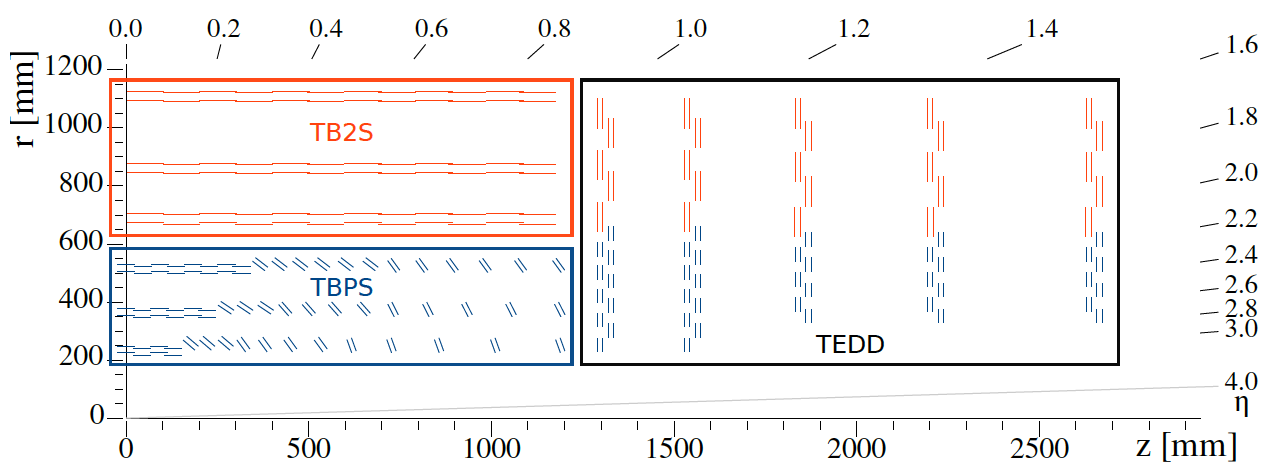
\includegraphics[width=.9\linewidth]{tex/Part2/fig/OT/OT-longitudinal.png}
\end{subfigure}
\caption{
  Longitudinal view of the CMS Phase II Outer Tracker layout  with two regions in the barrel (TB2S, TBPS) and the endcap region (TEDD).
  For the luminosity measurement only the barrel outermost layer 6 in the TB2S part is used, this layer consists of 78 sensor ladders on each side of CMS.
}
\label{fig:OT_layout}
\end{figure}


\begin{figure}[hbtp]
\centering
\begin{subfigure}
  \centering
  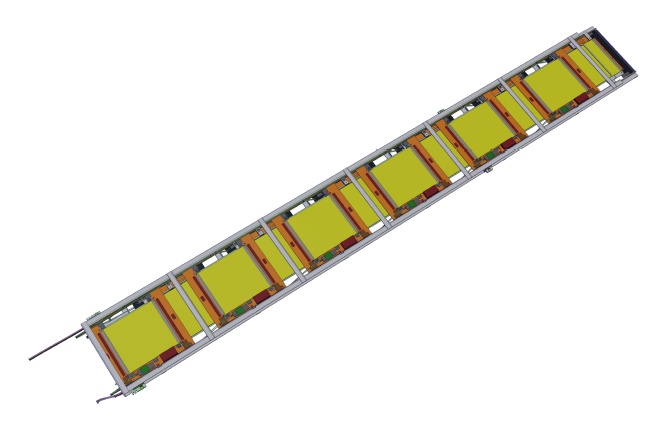
\includegraphics[width=.48\linewidth]{tex/Part2/fig/OT/OT-ladder.png}
\end{subfigure}
\begin{subfigure}
  \centering
  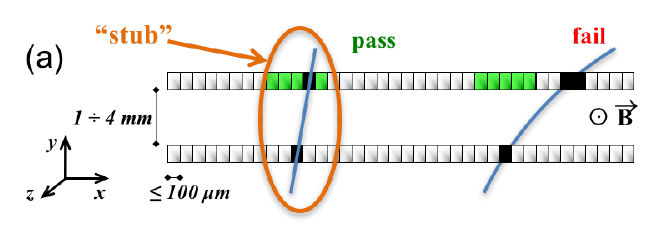
\includegraphics[width=.48\linewidth]{tex/Part2/fig/OT/OT-stub.png}
\end{subfigure}
\caption{
  Layout of one OT sensor ladder with 12 modules (left) and diagram of the track stub reconstruction (right) using the two sensor layers in each module.  
}
\label{fig:OT_ladder_stub}
\end{figure}


\begin{figure}[hbtp]
\centering
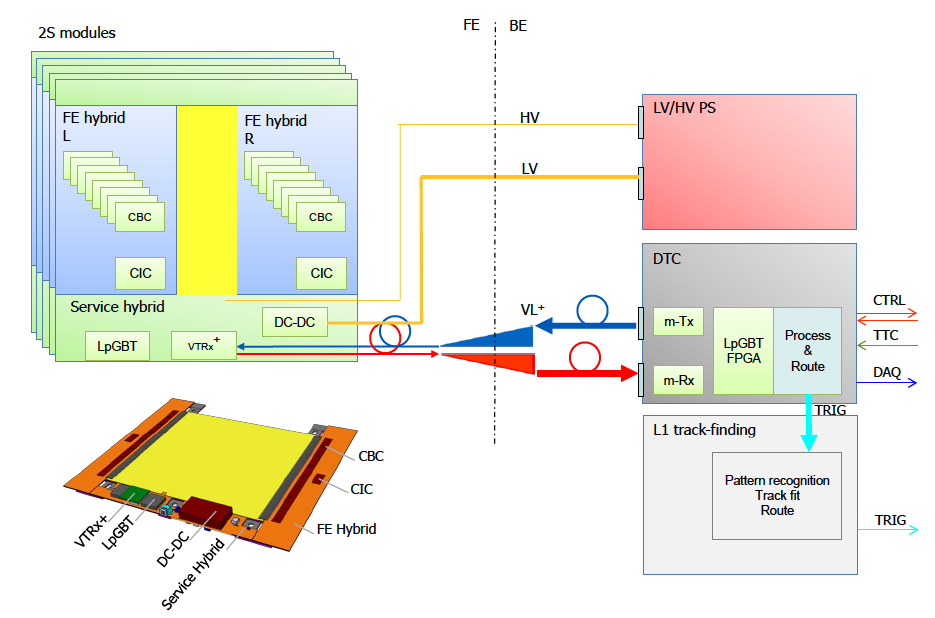
\includegraphics[width=.65\linewidth]{tex/Part2/fig/OT/OT-DAQoverview.png}
\caption{
  Design of the Phase II Outer Tracker frontend (FE) and backend (BE) electronics~\cite{CERN-LHCC-2017-009}.  
}   
\label{fig:OT_DAQ}
\end{figure}


\begin{figure}[hbtp]
\centering
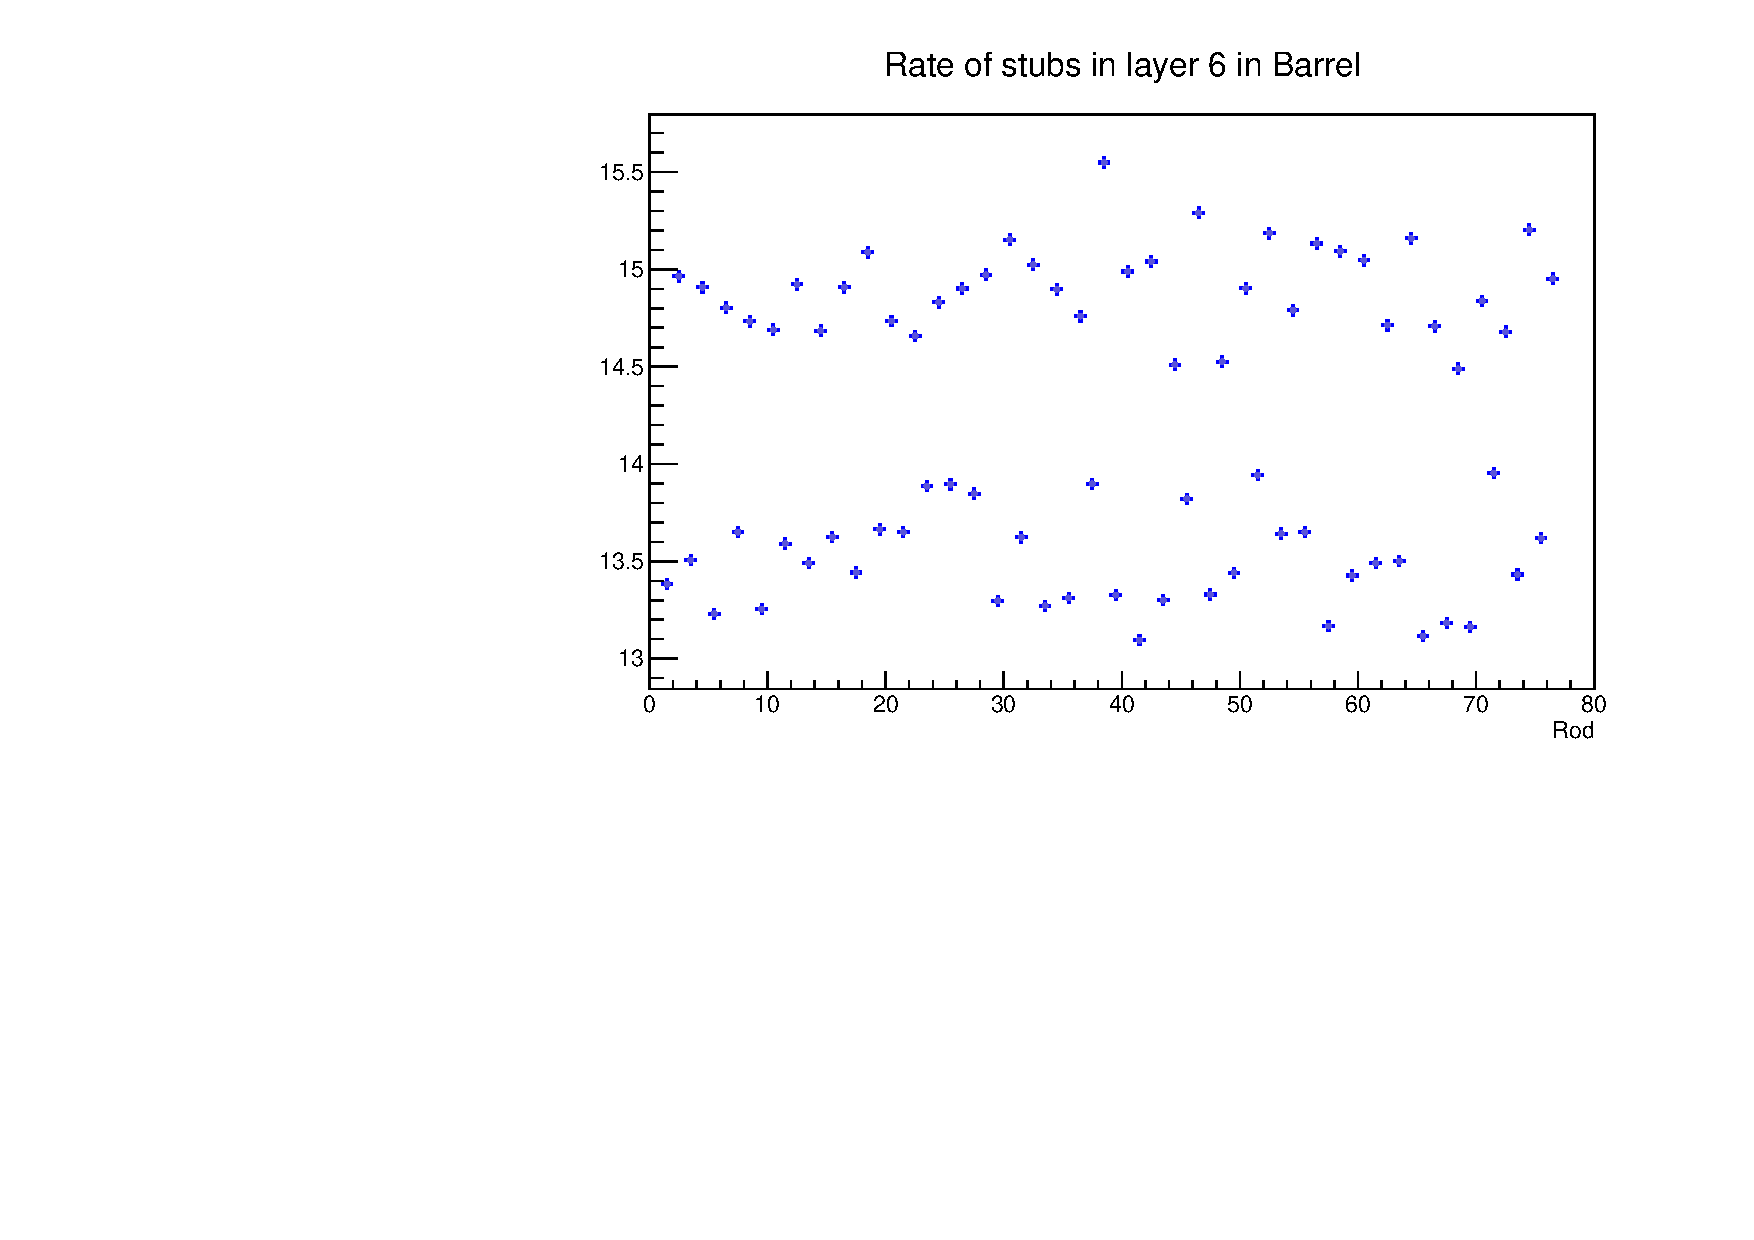
\includegraphics[width=.6\linewidth]{tex/Part2/fig/OT/OT-Rates.pdf}
\caption{
  Average number of track stubs per event per ladder as a function of the ladder id.
  The rate is determined from the CMS Phase II simulation for a pile-up of 200.
}
\label{fig:OT_rates}
\end{figure}


\begin{figure}[hbtp]
\centering
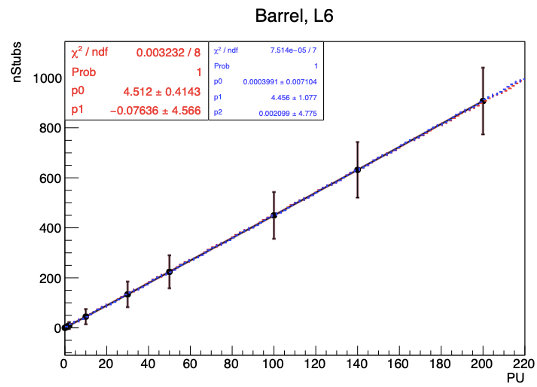
\includegraphics[width=.6\linewidth]{tex/Part2/fig/OT/OT-linearity.png}
\caption{
 Average number of track stubs per event as a function of pile-up determined from the CMS Phase II simulation showing a linear behaviour.
} 
\label{fig:OT_linearity}
\end{figure}

%\chapter{Luminosity Trigger Generation and Special Clocking Scheme}
\chapter{\textcolor{red}{Muon Drift Tube Luminometer}}
\label{sec:DT-lumi}
%%
%%For muon trigger stub counting, the use of trigger scouting methods prototyped at the end of Run 2
%%will allow per-bunch emittance scan analysis as well as luminosity measurement in physics conditions.
%%Muon trigger stub counting in Run 2 was orbit-integrated at per-LS frequency in real time;
%%using trigger scouting online bunch-by-bunch measurement at 4LN frequency is targeted in Run 3.
%%
%%It is also foreseen to ... expand the muon DT and resistive plate chamber (RPC) functionality to provide bunch-by-bunch
%%trigger primitives instead of a value integrated over a complete orbit.
%% orbit-integrated DT muon stub counting in Run 2 was available in real time at LS frequency.
%%
%%In Run 2, techniques like the DT muon trigger stub counting and the RAMSES radiation monitoring have proven
%%to be useful for stability and linearity studies, and they are planned to be exploited also in Phase-2.
%%To alleviate some of the limitations and allow per-bunch measurements, there is a requirement for Phase-2
%%for the upgrade of the muon counting for luminosity to have a 40MHz readout, as described in Section 7.4.2.
%%
%%In Run 2, counting of track candidates in the barrel muon systems has been shown to have good
%%linearity and can be used for stability and linearity monitoring of other luminometers. The CMS
%%DT chambers are installed in the return barrel yoke and provide muon tracking and triggering
%%for CMS physics operation. The observable used in both Run 1 and Run 2 was the barrel sorter
%%rate from the barrel muon track finder (BMTF), which counts muon track candidates with lumi
%%section granularity, but integrated over all bunches in the orbit. The statistical uncertainty
%%in the orbit-integrated rates at a luminosity of 2 x 1034 cm2 s1 is 0.2\%.
%% Assuming a fill of 2544 equally populated colliding bunches, the statistical uncertainty per BX would be 12%.
%% A naive extrapolation to a total luminosity of 51034 cm2 s1 for HL-LHC yields a statistical
%% uncertainty per BX of 8%.
%%
%%Drift tube muon system: As mentioned, the current implementation of DT luminosity
%%is extremely useful, but it does not provide the necessary statistical precision and
%%time granularity to meet Phase-2 requirements. Thus the rates and statistical uncertainties
%%achievable with different levels of muon trigger objects need to be studied
%%in detail to identify the most suitable one for a 40MHz precision online measurement.
%%The possibility of using the DT back-end electronics for dedicated luminosity
%%processing during Run 3 should be investigated.
%%

During Run 2, counting of muon track candidates from the CMS Level 1 trigger system, the Barrel Muon Track Finder (BMTF),
has proven to be useful for the luminosity systematics estimation due its excellent linearity and stability \cite{LUM-17-001}.
The observable used was the barrel track sorter rate integrating BMTF track candidates over the entire orbit and over one lumi section ($\sim$23 s) period.
%The statistical precision of this counter for the Run 2 instantaneous luminosity of  $2\times10^{34}\ \text{cm}^{-2}\text{s}^{-1}$ was of order 0.2\% per orbit per lumisection.
This counter was recorded by the BRILDAQ in real time and had a statistical precision of about 0.2\% per orbit per lumi section for the Run 2 instantaneous luminosity of  $2\times10^{34}\ \text{cm}^{-2}\text{s}^{-1}$.
%however was of limited use for online luminosity measurement due to the lack of per bunch information and relatively long integration time.
The  uncertainty with the BMTF tracks at the HL-LHC instantaneous luminosity of $7.5\times10^{34}\ \text{cm}^{-2}\text{s}^{-1}$
is expected to be of the order of 25\% per bunch per second, which does not provide enough precision for an online luminometer.
Below we describe an improved luminometer design based on muon trigger primitives which will be available 
from the Phase-2 back end of the barrel detector for each of the Muon Drift Tube (DT) chambers, and provides higher count rates per bunch crossing.


\section{Detector Description and Trigger Primitives}

The Muon DT chambers are installed in the barrel yoke of the CMS detector \cite{DT-2009}.
A total of 250 chambers are distributed in 5 wheels (YB=0,$\pm$1,$\pm$2) and four radial layers (MB=1-4),
a layout of the entire  CMS muon system is shown in Figure~\ref{fig:DT_layout}.
The RPC chambers are also visible in this diagram as layers RB1-RB4 in front of the DT chambers.

Hits from the DT, RPC, and HO detectors will be combined to reconstruct muon track segments (trigger primitives)
per DT chamber as part of the  Level 1 muon reconstruction system in Phase-2 \cite{CERN-LHCC-2017-012}.
The rates of these trigger primitives have been studied using Run 2 data.
Figure~\ref{fig:DT_rates} shows the rates for the YB+2  chambers,
the values have been extrapolated up to the expected HL-LHC instantaneous luminosity
of  $7.5\times10^{34}\ \text{cm}^{-2}\text{s}^{-1}$ from the measured values in Run 2 data.
We observe that the chambers in the first radial layer MB1 detect the highest rate
and the rate decreases to less than 10\% at the outermost layer,
this behaviour is consistent with a significant contribution of particles from jet punch-through observed by the inner layers.
In the MB4 layer we observe a phi asymmetry with higher rates on the top of the CMS detector (Sectors 3-5), believed to be due to neutron backgrounds,
for this reason we expect to exclude this layer from the final luminosity calculation as the rates are not expected to always scale linearly with the number of IP collisions. 




\begin{figure}[hbtp]
\centering
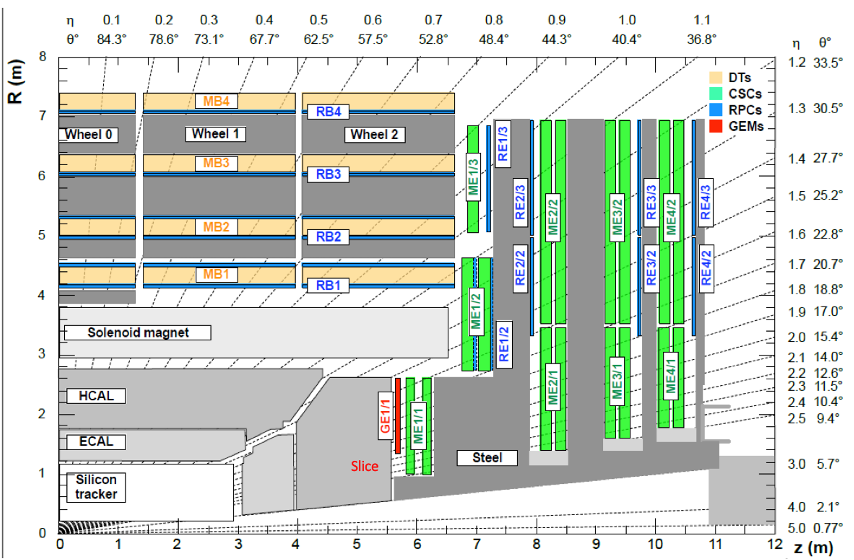
\includegraphics[width=.8\linewidth]{tex/Part2/fig/DT/DT-longitudinal.png}
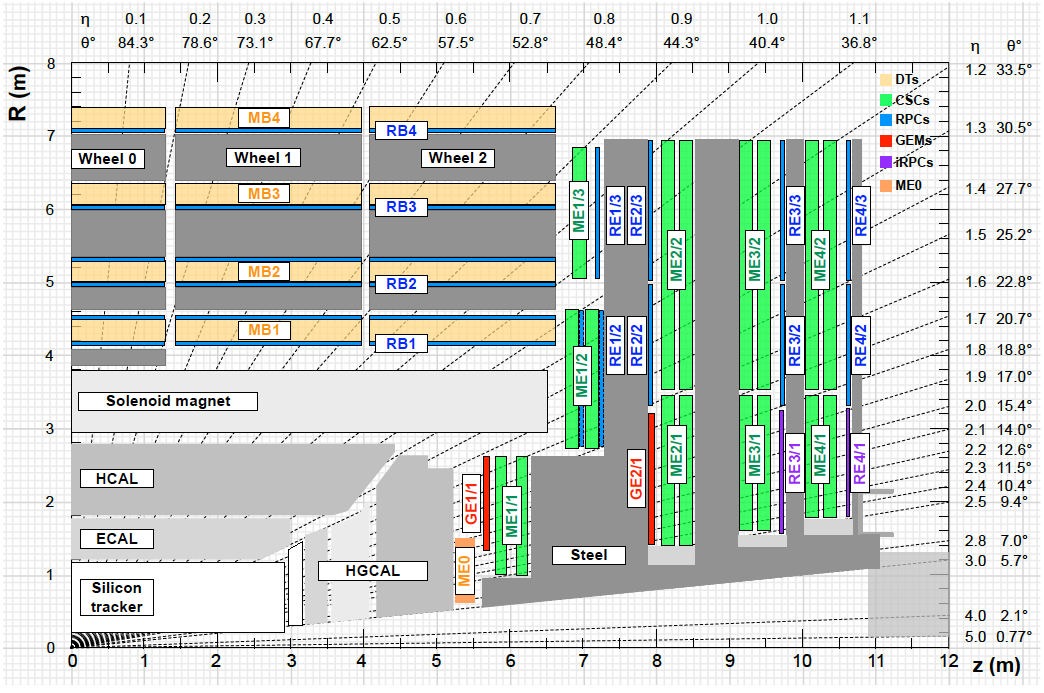
\includegraphics[width=.7\linewidth]{tex/Part2/fig/DT/DT-transverse.png}
\caption{
  Longitudinal view of one quarter of the CMS muon detector system (top) showing the Drift Tube chambers in the barrel region
  and transverse view (bottom) showing the 12 phi sectors and a muon track trayectory.
  The numbering scheme for the chambers is shown within the figure and consists of a wheel number, a radial station number (MB), and phi sector.
}
\label{fig:DT_layout}
\end{figure}

\clearpage

\section{Data Acquisition}

The muon system readout electronics will undergo a complete upgrade for Phase-2 in order to cope with the higher data rates and L1 trigger demands.
Figure~\ref{fig:DT_DAQ2} shows a comparison of the current components of the DT back end and the new architecture for Phase-2 \cite{CERN-LHCC-2017-012}.
In the Phase-2 design, the front-end electronics are upgraded with On-Board Electronics for DT (OBDT) in new Minicrate 2 boards based on FPGA's.
The data, including the full collection of DT, RPC, and HO hits, will be continously streamed via high speed optical
links to the back-end Layer 1 processor boards (L1 processors) where the trigger primitives are reconstructed.
The L1 processors will consist of ATCA boards capable of processing full DT phi sectors, approximately 60 processor boards in total,
and will allow for significant improvements in the trigger primitive reconstruction including improved bunch crossing identification
through improved timing resolution as well as improved spatial resolution. 


For the online luminosity measurement, the BRIL Histogramming firmware described in Chapter~\ref{sec:BRILDAQ}
operating in synchronous mode will be installed as part of the back-end Layer 1 processor firmware.
This histogramming module will access and count the list of trigger primitives in parallel to the CMS L1 trigger stream
and produce a histogram with counts per bunch crossing (3564 bins) at approximately 1 second integration intervals.
Based on the expected number of trigger primitive counts per bunch crossing, the required memory per histogram is estimated at 28 Kb,
requiring a minimal amount of the L1 processor resources. 
The histograms  will be transferred to the BRILDAQ system as part of the IPBus network traffic used for the slow control the DT back-end.
The total data rate expected for the DT luminometer (250 histograms) at the BRILDAQ end is aproximately 7.1 Mbps.
As for the other luminometers, the individual histograms will be merged inside the BRILDAQ accounting for possible background subtraction and filtering of any misbehaving chambers.
%Due to dependence on the CMS L1 trigger system, this luminometer will operate only during stable beams.
\textcolor{red}{(here need a sentence about the availibility of this luminometer, e.g. when the HV will be ON, DAQ configured and trigger primitives generating, and lumi nibble counter for histogram reset)}

A demonstrator of the DT Phase-2 electronics has been installed in one sector (YB+2, S12) to take data during Run 3.
A total of 12 OBDT's were installed in the four MB layers, with the MB 3 and 4 equiped with a dual readout using both OBDT's and Legacy electronics.
A back-end prototype (AB7) based on legacy TwinMux boards is currently used for event matching and trigger primitive generation.
Since 2020, a test version of the BRIL Histogramming firmware has been installed in the AB7 back end and is expected to record data during Run 3.


\begin{figure}[hbtp]
\centering
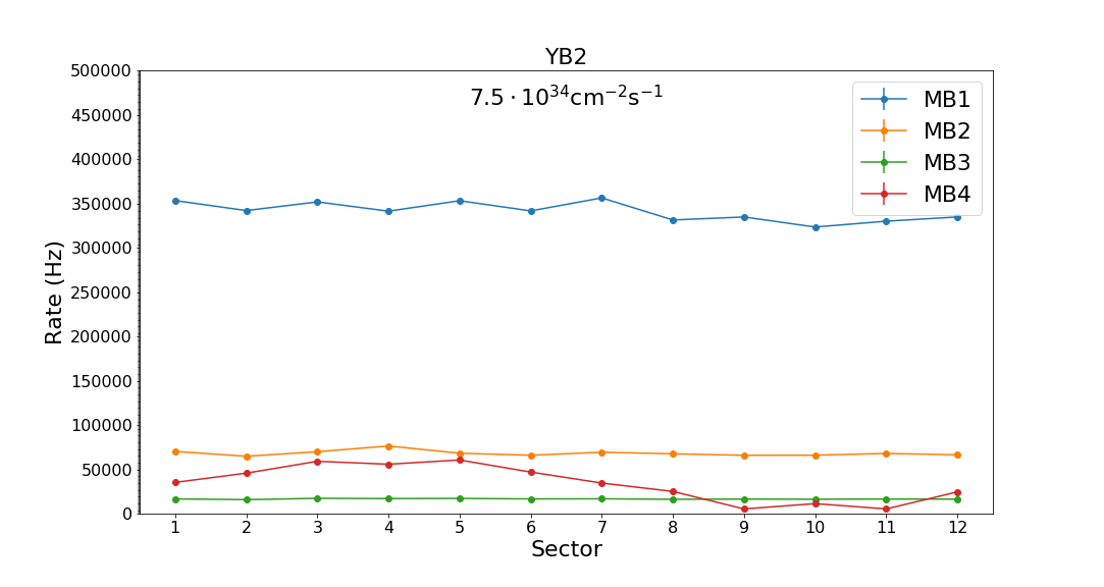
\includegraphics[width=.8\linewidth]{tex/Part2/fig/DT/DT-RatesExtrapolated.png}
\caption{L1 trigger primitive rates expected for HL-LHC instantenous luminosity conditions for the DT chambers in the wheel YB+2\textcolor{red}{(check if RPC/HO hits are included here)}.} 
\label{fig:DT_rates}
\end{figure}

\begin{figure}[hbtp]
\centering
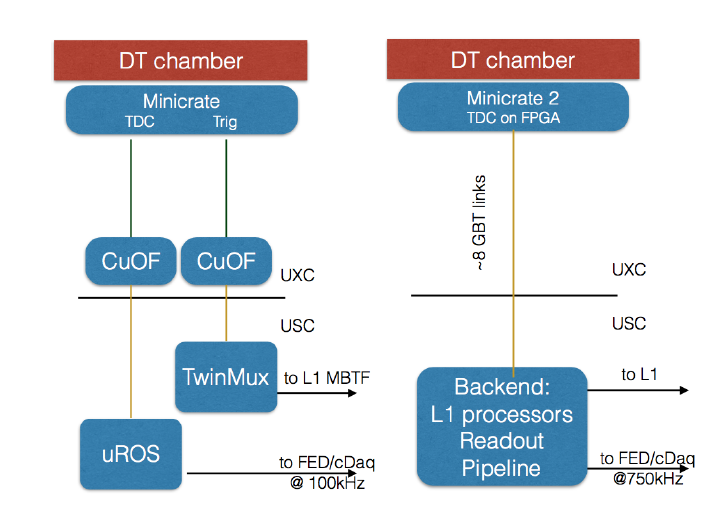
\includegraphics[width=.7\linewidth]{tex/Part2/fig/DT/DT-DAQ-Phase1_vs_Phase2.png}
\caption{Current partition of the DT system readout electronics (left) and Phase-2 upgrade design (right) using On-Board Electronics for DT (OBDT).
  The muon trigger primitives are produced by the L1 processors.
}   
\label{fig:DT_DAQ2}
\end{figure}


\clearpage

\section{Expected Performance}

Despite the increased particle rates at the HL-LHC conditions, the expected hit occupancy for the DT chambers will remain low at about 50 Hz cm$^{-2}$
and below 500 kHz per station at the inner MB layers.
At these rates the counting of trigger primitives should remain linear up to high pileup, a necesary property for precision luminosity measurement.
Figure~\ref{fig:DT_linearity} shows the dependence of the number of DT trigger primitives on the instantenous luminosity
observed using Run 2 data up to about $2\times10^{32}$ cm$^{-2}$ s$^{-1}$.
A very linear behaviour is observed, the deviations from linearity obtained from this data are less than \textcolor{red}{ XX\%}.

Another important aspect is the statistical precision during normal Physics running as well as during the vdM scans used to obtain the calibration constant.
To estimate the statistical precision we use the trigger primitive rates previously extrapolated to the HL-LHC luminosity conditions.
Excluding the MB4 layer, the total orbit integrated rate expected is $\sim$17 MHz at $7.5\times10^{34}$ cm$^{-2}$ s$^{-1}$;
this corresponds to about 0.61 trigger primitives per bunch crossing for Physics and 0.00153 per bunch crossing for vdM conditions.    
For the online luminosity measurement, using one colliding bunch and 1 s integration period for Physics (30 s for vdM),
the statistical precision expected is 1.2\% (4.4\%).
During Physics conditions the expected statistical precision meets the requirement of 2\%,
while for vdM a precision of 0.36\%  meeting the requirements for the calibration constant (1\%) will be obtained only after combining all colliding bunches, 150 assummed here.
The final precision of this luminometer will depend additionally on the ability to handle any backgrounds and keep a stable operation of the muon detector and DAQ over entire run periods.


%\begin{figure}[hbtp]
%\centering
%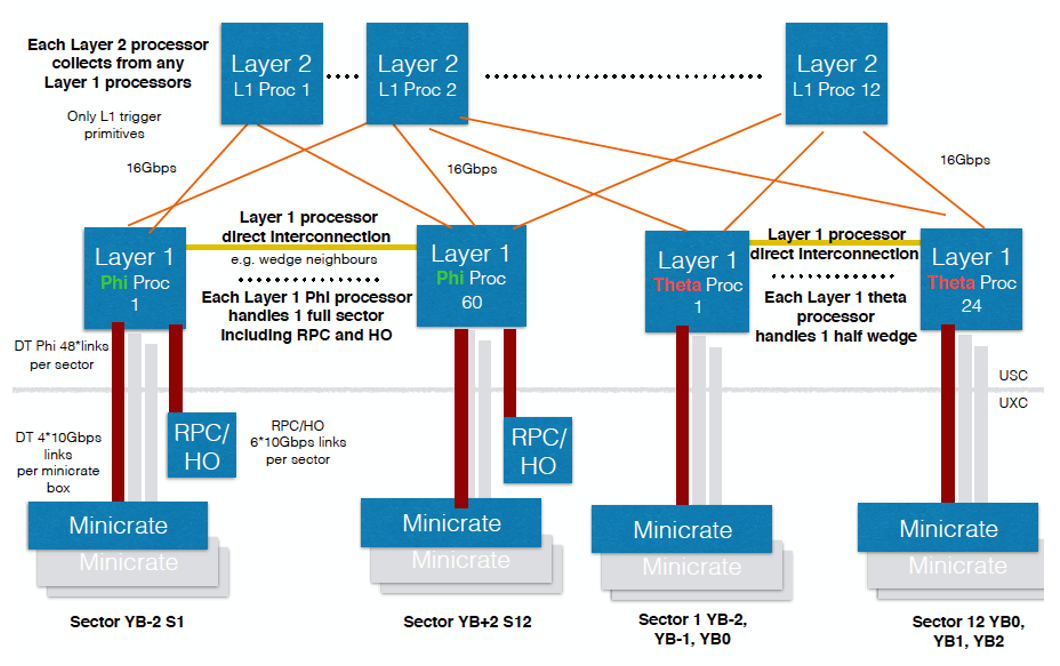
\includegraphics[width=.65\linewidth]{tex/Part2/fig/DT/DT-DAQoverview.png}
%\caption{Design  of the Muon DAQ system architecture for Phase II showing the different layers where the L1 trigger objects are generated. In  this layout the DT trigger primitives are generated in the Layer 1 of the backend.}   
%\label{fig:DT_DAQ}
%\end{figure}


\begin{figure}[hbtp]
\centering
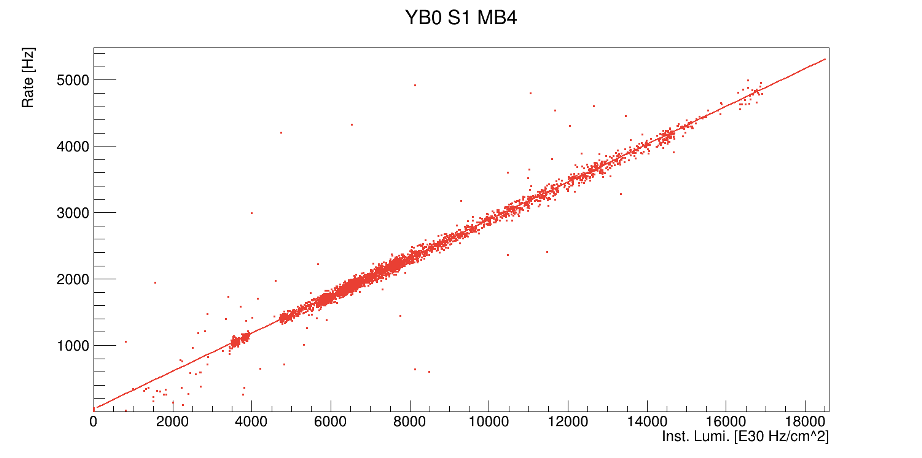
\includegraphics[width=.49\linewidth]{tex/Part2/fig/DT/DT-Linearity.png}
\includegraphics[width=.35\linewidth]{tex/Part2/fig/DT/DT-Linearity-residuals.png}
\caption{L1 trigger primitive rates for one DT chamber ( \textcolor{red}{YBXX-MBXX-SXX}) as a function of instantenous luminosity (left) measured in one Physics run during 2018
and relative deviations from the linear fit (right).} 
\label{fig:DT_linearity}
\end{figure}



%\chapter{Trigger Scouting System Luminosity}
%\chapter{Beam Halo Monitor}
%\chapter{Additional Radiation and Neutron Monitors}

\section{RAMSES}

\section{LHC RADMON}

\section{RadFET}

\section{PIN diode}
%\chapter{BRIL Data Acquisition System}

%Part III
%\part{Project Organisation, Responsibilities, Planning \& Cost}
%\chapter{Project Organisation}
%\chapter{Institutional Interests and Responsibilities - Task Sharing}
%\chapter{Project Schedule and Milestones}
%\chapter{Cost Estimate}
%\chapter{Risk Analysis}

%% **DO NOT REMOVE BIBLIOGRAPHY**
\bibliography{briltdr2021}   % will be created by the tdr script.
%% examples of appendices.
%\clearpage
%\appendix
%\section{Appendix name}
%%% DO NOT ADD \end{document}!

